%% Not a title: a legend row above the axes carries its line samples.
\documentclass[border=0pt]{standalone}
\usepackage{tikz}
\begin{document}
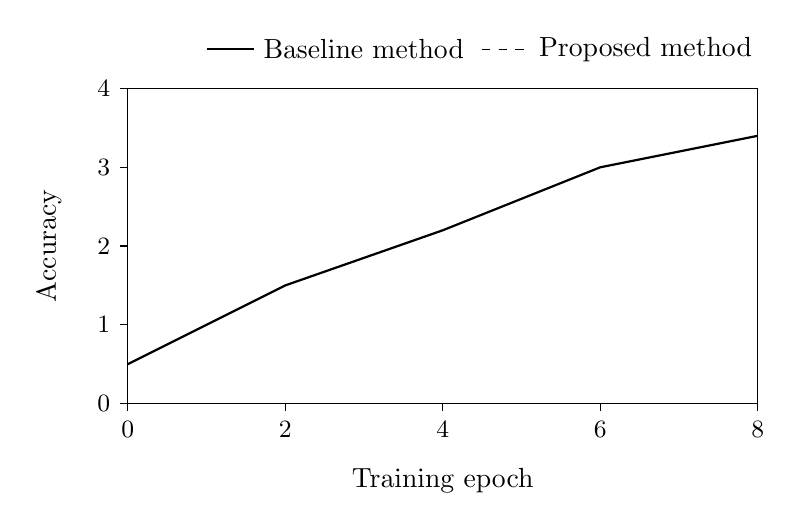
\begin{tikzpicture}[every node/.style={font=\fontsize{9}{11}\selectfont}]
\draw (0,0) rectangle (8,4);
\draw[thick] (0,0.5) -- (2,1.5) -- (4,2.2) -- (6,3) -- (8,3.4);
\foreach \x in {0,2,4,6,8} {\draw (\x,0) -- (\x,-0.1); \node[below] at (\x,-0.1) {\x};}
\foreach \y in {0,1,2,3,4} {\draw (0,\y) -- (-0.1,\y); \node[left] at (-0.1,\y) {\y};}
\node[below] at (4,-0.7) {\fontsize{10}{12}\selectfont Training epoch};
\node[rotate=90] at (-1.0,2) {\fontsize{10}{12}\selectfont Accuracy};
\draw[thick] (1,4.5) -- (1.6,4.5); \node[right] at (1.6,4.5) {\fontsize{10}{12}\selectfont Baseline method};
\draw[dashed] (4.5,4.5) -- (5.1,4.5); \node[right] at (5.1,4.5) {\fontsize{10}{12}\selectfont Proposed method};
\end{tikzpicture}
\end{document}
